\recipe[]{Negroni \& derivati}
\serves{1}%<----Numero di porzioni
\preptime{5 minuti}%<---Tempo di preparazione
\cooktime[]{-}%<-----Tempo di cottura
\autore{Max}
\begin{ingreds}
\ingredients[Negroni]
	50ml Gin \index{gin}
	50ml Vermouth rosso \index{vermouth}
	50ml Bitter \index{bitter}
	1 fetta d'arancia \index{arancia}
	Scorza d'arancia
	2 gocce di angostura (opzionali) \index{angostura}

\columnbreak

\ingredients[Americano:]
	Sostituisci Gin con Tonica
\ingredients[Sbagliato:]
	Sostituisci Gin con Prosecco
\ingredients[Milano-Torino:]
	Togli Gin
\ingredients[Garibaldi:]
	Sostituisci Gin e Vermouth con Succo d'arancia

\end{ingreds}

\begin{method}
Metti il giaccio in un bicchiere old fashioned, versa tutti gli ingredienti e mescola leggermente. Inserisci nel bicchiere una fetta d'arancia e spruzza un po' di scorza di arancia sul bicchiere per profumarlo.

La lista degli ingredienti comprende il Negroni e le variazioni per produrre i derivati. Seguendo lo schema della figura \ref{negroni:schema} è facile produrre tutte le varianti, ricordando queste regole: il bicchiere è old fashioned, gli ingredienti vanno divisi in parti uguali, la tonica va aggiunta per ultima.
\end{method}

%\subsection*{Note}

% Figura
\begin{figure}[!h]
\centering
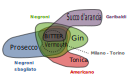
\includegraphics[]{img/negroni.png}
\caption{Il Negroni e i suoi derivati.}
\label{negroni:schema}
\end{figure}



